\subsection{Diodi} 
L'esperienza è cominciata con lo studio del comportamento di alcuni diodi, sfruttando il circuito \ref{fig:cD}.

\begin{figure}[h]
    \begin{center}
    \begin{circuitikz} []
    \draw
        (0,2) to [battery] (0,0)
        (0,0) to (3,0)
        (0,2) to [ammeter] (2,2) 
        (2,2) to [Do] (2,0)
        (2,2) to (3,2)
        (3,2) to [open, *-*] (3,0);
    \end{circuitikz}
    \caption{Circuito usato per l'analisi dei diodi}
    \label{fig:cD}
    \end{center}
\end{figure}

Per ognuno dei quattro diodi a nostra disposizione abbiamo preso le misure di come varia $i$ in funzione di $\Delta V$. Qui esponiamo solo i dati di uno dei diodi, per evitare di ripetere sempre le stesse cose. I valori che otteniamo rappresentano una curva che assomiglia ad un'esponenziale, per cui proviamo a linearizzare il grafico. Ciò che otteniamo sono i due grafici riprodotti in figura \ref{fig:gDe} e \ref{fig:gDl}. 

\begin{figure}
    \centering
    \begin{minipage}{0.5\textwidth}
        \centering
        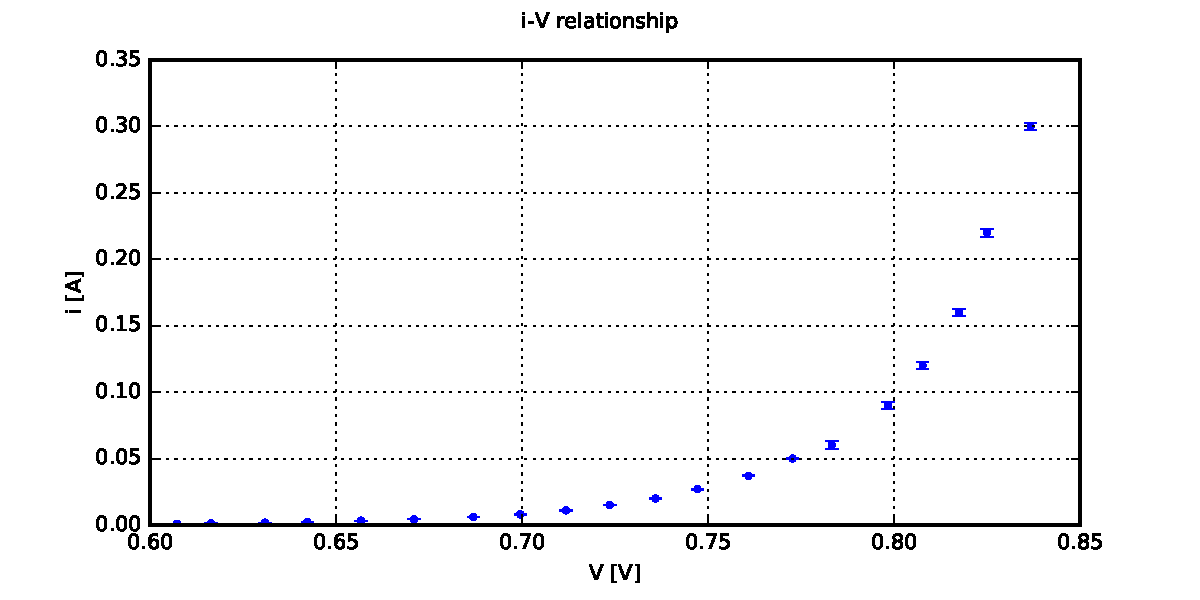
\includegraphics[width=\textwidth]{fig1D.pdf} 
        \caption{Grafico esponenziale di $i$ in funzione di $\Delta V$}
        \label{fig:gDe}
    \end{minipage}\hfill
    \begin{minipage}{0.5\textwidth}
        \centering
        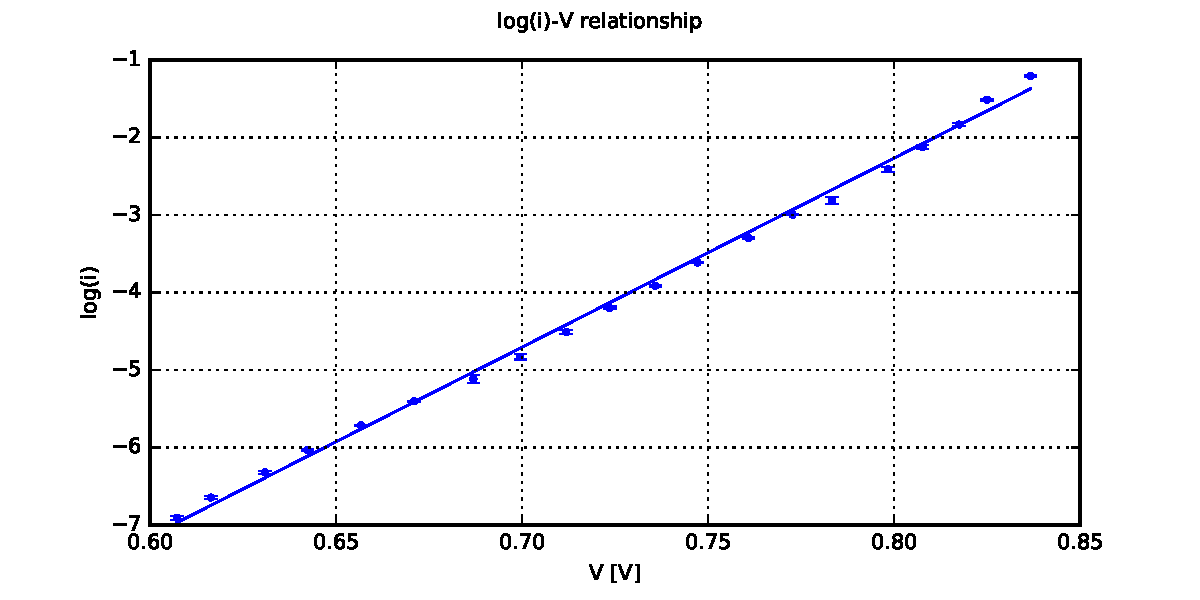
\includegraphics[width=\textwidth]{fig2D.pdf} 
        \caption{Grafico linearizzato di $\ln{i}$ in funzione di $\Delta V$ con relativo modello}
        \label{fig:gDl}
    \end{minipage}
    
\end{figure}
    
Proviamo quindi a cercare i parametri della retta ottenuta linearizzando il grafico attraverso una regressione lineare. Assumiamo che l'incertezza di $\Delta V$, cioè dovuta al DMM sia nulla. Mentre per trovare l'incertezza su $i$, $\sigma[i]$, assumiamo che all'interno dell'intervallo di incertezza massimo ci sia equiprobabilità tra tutti i possibili valori, per cui non possiamo sapere niente. Ovviamente quindi a seconda del fondo scala preso in considerazione varia l'incertezza sulla misura, che sarà cioè maggiore per i valori aventi una corrente più elevata. Per ottenere i valori di intercetta e pendenza prendiamo il grafico di $\Delta V$ in funzione di $i$, e a partire da esso quello di $\Delta V$ in funzione di $\ln{i}$. Attraverso il metodo dei minimi quadrati troviamo ora i valori di intercetta e pendenza di questo grafico, che chiameremo $A_p$ e $B_p$ rispettivamente. Ora non ci resta che invertire gli assi e propagare le incertezze sui nuovi parametri della retta e otteniamo il modello che descrive l'andamento, con dei valori $A$ e $B$ definitivi. \\

\begin{gather}
    \sigma[V]=0 \quad \sigma[i]= \frac{I_{FS}}{50 \sqrt{12}} \quad \sigma[\ln{i}] = \frac{\sigma[i]}{i}
    \\
    B = \frac{1}{B_p} = 24 \quad A = - A_p B = -21.8
    \\
    \sigma[B] = \frac{\sigma[B_p]}{B_p^2} = 1 \quad \sigma[A] = \sqrt{(B \sigma[A_p])^2 + (A_p \sigma[B])^2} = 0.9
    \\
    \label{eq:regr1}
\end{gather}

A parte qualche punto che si discosta un po' più degli altri osserviamo quindi che il modello descrive abbastanza bene i dati ottenuti. Infatti tutti i punti rientrano entro al massimo un $3\sigma$ dal modello, a parte solo l'ultimo. Perciò i valori di $i$ in funzione di $\Delta V$ seguono effettivamente un andamento esponenziale. \\
Un risultato analogo si è ottenuto anche per gli altri tre diodi da noi studiati. \\ \\

Consideriamo ora il diodo Zener, e studiamo il suo comportamento in modo analogo a quanto fatto con i diodi, sebbene con le dovute dovute alle differenti modalità di misura da noi adottate. In particolare il circuito da noi considerato è quello rappresentato in figura \ref{fig:cZ}

\begin{figure}[h]
    \begin{center}
    \begin{circuitikz} []
    \draw
        (0,2) to [battery] (0,0)
        (0,0) to (3,0)
        (0,2) to [ammeter] (2,2) 
        (2,0) to [zzDo] (2,2)
        (2,2) to (3,2)
        (3,2) to [open, *-*] (3,0);
    \end{circuitikz}
    \caption{Circuito usato per l'analisi dei diodi Zener}
    \label{fig:cZ}
    \end{center}
\end{figure}

Anche in questo caso studiamo $i$ in funzione di $\Delta V$ e ancora usiamo le stesse modalità per trovare i valori a cui siamo interessati. I calcoli sono li stessi di prima, perciò qui forniamo solo i risultati numerici.

\begin{gather}
    B = 4.30 \quad A = -25.3
    \\
    \sigma[B] = 0.04 \quad \sigma[A] = 0.3
    \\
    \label{eq:regr2}
\end{gather}

Andiamo quindi a studiare i grafici che otteniamo e osserviamo se il modello rispetto la previsione teorica. I grafici che otteniamo sono \ref{fig:gZe} e \ref{fig:gZl}

\begin{figure}
    \centering
    \begin{minipage}{0.5\textwidth}
        \centering
        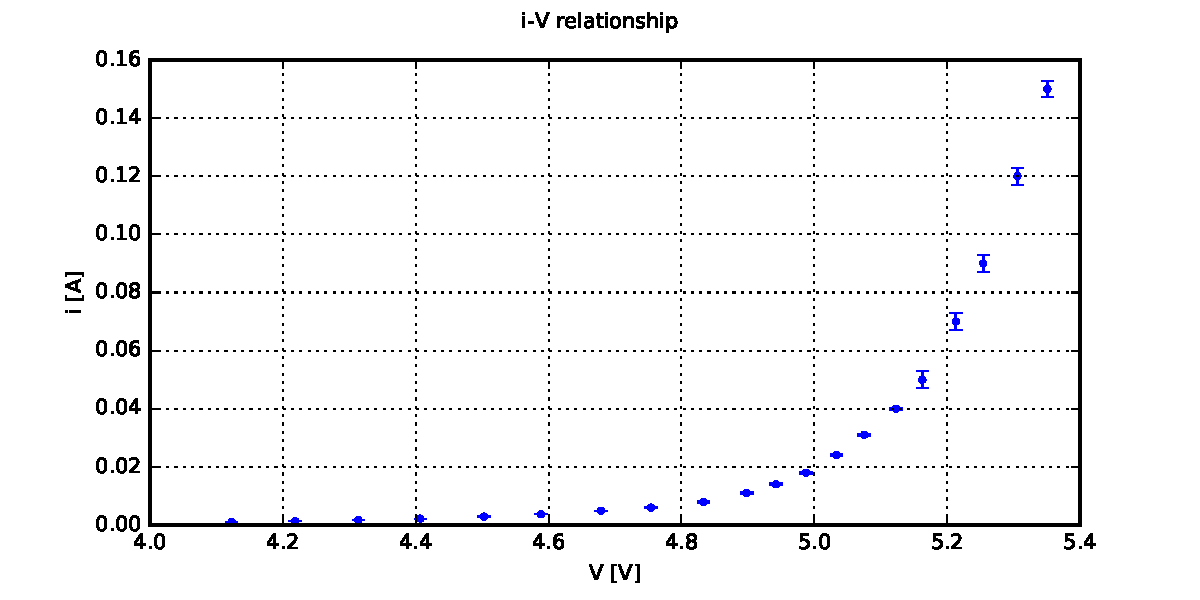
\includegraphics[width=\textwidth]{fig1Z.pdf} 
        \caption{Grafico esponenziale di $i$ in funzione di $\Delta V$}
        \label{fig:gZe}
    \end{minipage}\hfill
    \begin{minipage}{0.5\textwidth}
        \centering
        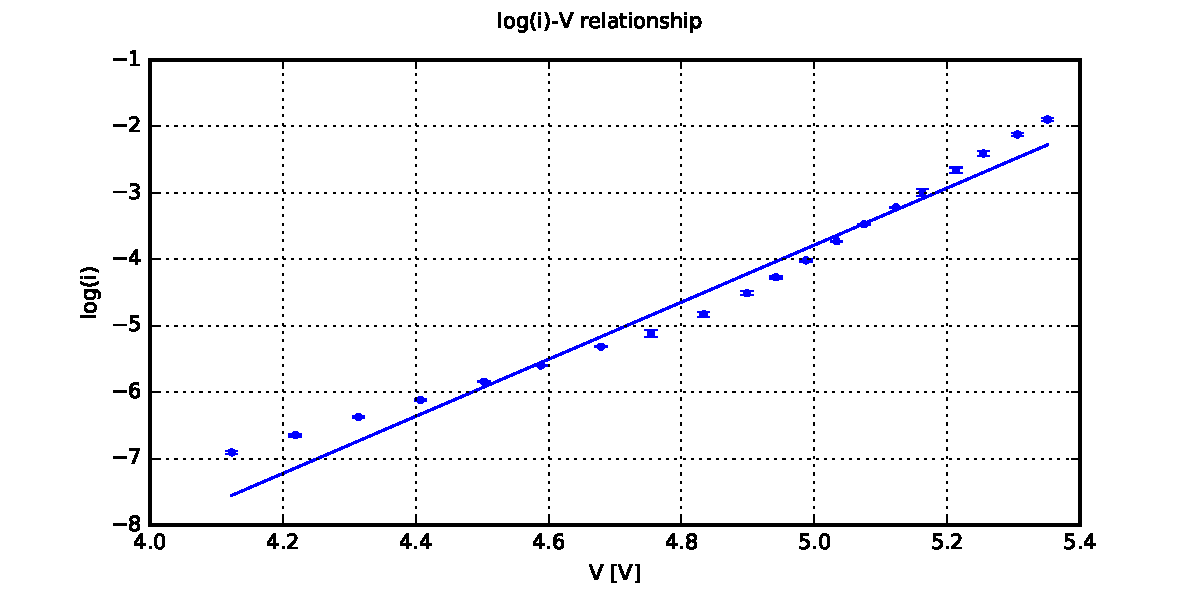
\includegraphics[width=\textwidth]{fig2Z.pdf} 
        \caption{Grafico linearizzato di $\ln{i}$ in funzione di $\Delta V$ con relativo modello}
        \label{fig:gZl}
    \end{minipage}
\end{figure}

Si nota tuttavia che nel grafico linearizzato i valori non risultano compatibili. In particolare sono rappresentate due semirette, spezzate in concomitanza del punto numero 9 della serie. Si suppone che in quel particolare punto sia successo qualcosa, plausibilmente è stato toccato il circuito e ciò ha provocato una variazione dei parametri. Si cercano quindi due nuovi modelli in grado di descrivere l'andamento dei punti prima e dopo questo punto. I nuovi parametri che si ottengono sono A1 e B1 per il primo tratto e A2 e B2 per il secondo. Li calcoliamo sempre allo stesso modo, per cui nuovamente inseriamo qui solo i risultati numerici finali.

\begin{gather}
    B_1 = 2.91 \quad A_1 = -18.9 \quad \sigma[B_1] = 0.08 \quad \sigma[A_1] = 0.5
    \\
    B_2 = 5.8 \quad A_2 = -32 \quad \sigma[B_2] = 0.2 \quad \sigma[A_2] = 1
    \\
    \label{eq:regr2}
\end{gather}

\begin{figure} [h!]
    \centering
    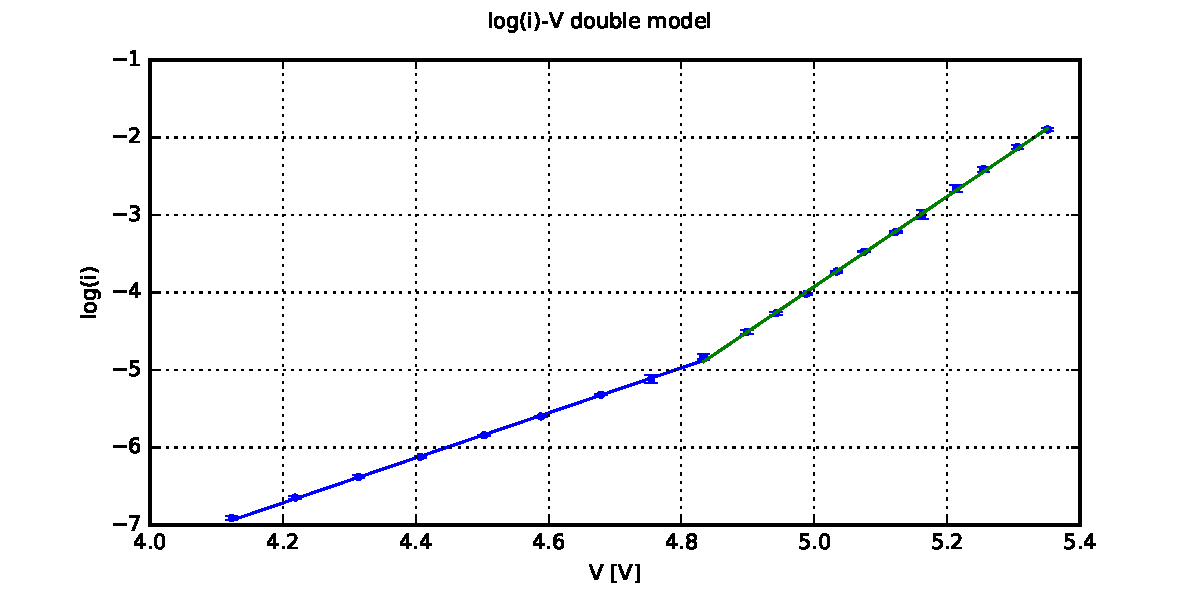
\includegraphics[width=\textwidth]{fig3Z.pdf} 
    \caption{Grafico di $\ln{i}$ in funzione di $\Delta V$ con i due modelli}
    \label{fig:gZc}
\end{figure}

Inseriamo quindi i nuovi valori all'interno di un grafico e osserviamo che questi due modelli descrivono alla perfezione i dati ottenuti nelle rispettive metà. Ciò avvalora dunque la tesi che effettuando la misura del punto 9 ci sia stata una modifica del circuito. Il grafico che otteniamo è \ref{fig:gZc}. \\ \\


Passiamo ora allo studio della resistenza dinamica. Essa rappresenta un valore tipico del diodo Zener che si modifica a seconda della corrente che scorre attraverso di esso ed alla differenza di potenziale a cui è sottoposto. Abbiamo in particolare deciso di studiare il suo comportamento in funzione della corrente. Otteniamo una curva che ha la forma di un'esponenziale. Per esserne certi consideriamo il logaritmo sia della corrente che della resistenza dinamica del nostro diodo e attraverso la regressione lineare osserviamo se ciò che otteniamo rappresenta o meno un andamento lineare. I valori che otteniamo sono i seguenti. Per quanto riguarda i risultati sulla regressione lineare non riscriviamo le formule, in quanto sempre le stesse. \\

\begin{gather}
    r_d = \frac{\Delta V}{i} \quad \sigma[r_d] = \frac{V \sigma[i]}{i^2} \quad \sigma[\ln{r_d}] = \frac{\sigma[r_d]}{r_d}
    \\
    A = -2.39 \quad B = -1.249 \quad \sigma[A] = 0.01 \quad \sigma[B] = 0.002
    \\
    \label{eq:regr3}
\end{gather}

Proviamo ad inserire quindi i risultati ottenuti nel grafico \ref{fig:gZr}, e troviamo quindi che l'andamento è rappresentato molto bene dalla retta da noi calcolata, avente i parametri sopra indicati. \\

\begin{figure} [h]
    \centering
    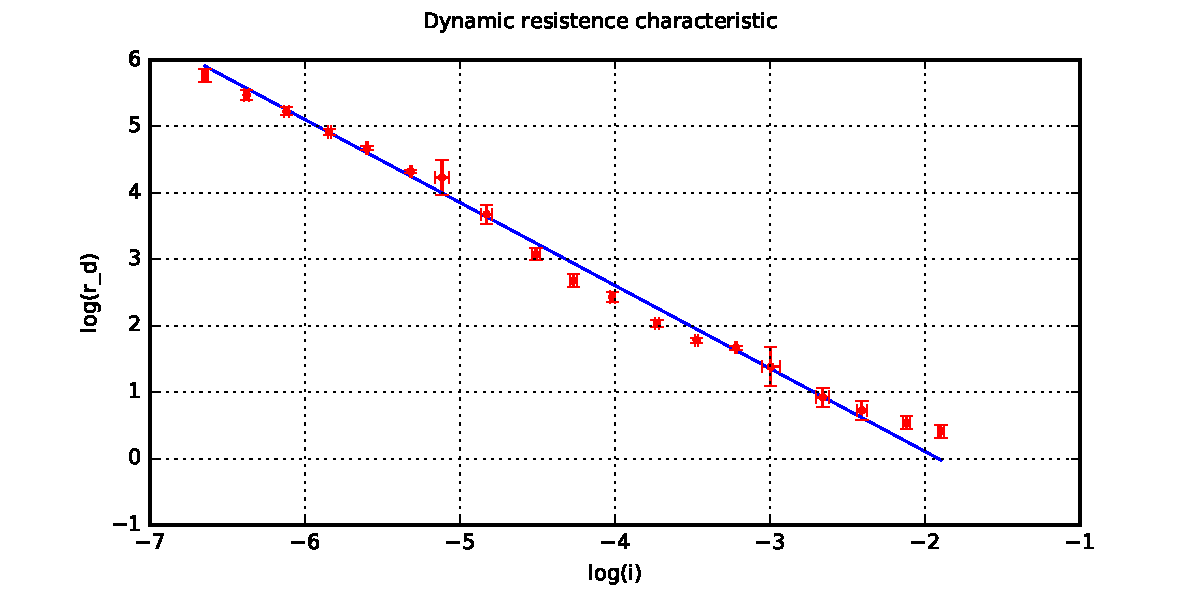
\includegraphics[width=\textwidth]{fig4Z.pdf} 
    \caption{Grafico di $\ln{r_d}$ in funzione di $\ln{i}$ con il relativo modello ottenuto tramite regressione lineare}
    \label{fig:gZr}
\end{figure}

Osserviamo inoltre che gli intervalli di incertezza di tutti i punti rientrano in almeno 3$\sigma$ dalla retta calcolata, per cui possiamo dire che effettivamente l'andamento da noi ottenuto risulta corretto. 